
\chapter{Boundary and Initial Conditions}\label{chp:boundary-and-initial}
The governing equations of fluid flow, their discretization and the forwards propagation in time of a solution have been discussed so far, but two more crucial elements that determine the problem have been neglected: initial conditions and boundary conditions of the system.

Without an initial condition to go on, most problems, especially if they don't solve for a steady-state solution, are undetermined. The solvers in \autoref{chp:solvers} calculate positions and velocities at a future time $t+\Delta t$ from the positions and velocities at the current time $t$ - seen backwards, this recursion must have an origin at some $t_0$ where positions and velocities are known. Constructing these positions and velocities for a given scenario that we wish to compute the dynamics of involves the act of discretizing a continuous field and might be thought of as trivial at a glance but actually has some nuances that determine the quality and stability in the first few seconds of the simulation - a timespan that can be of significant importance.

Boundary conditions are equally essential to the description of many problems, especially real-world problems that are full of complex boundary conditions and -geometry. Simulations that are actually boundless or where boundary conditions do not matter are typically not the most interesting. In some way or another, slip, no-slip, periodic or otherwise, the limits of the simulated domain must be enforced, desirably in the most robust and elegant way possible.

Both of these factors will be discussed in the following. In particular, a single layer of non-uniformly sampled particles will be used to represent boundaries, giving great flexibility while fitting seamlessly in the solvers developed in \ref*{chp:solvers}. Jittering of initial positions as a way of reducing aliasing and the stability of the initial lattice in which continua are discretized will be discussed. Finally, an iterative method for enforcing a uniform initial density field will be shown.

\section{Non-Uniform Single Layer Boundaries}

While a great many boundary handling methods for SPH exist, a very common idea is to use the same type of discretization for boundaries as for fluids and represent them as particles, even going so far as to reuse the pressure solver to compute contact forces\autocite*{versatile-boundary-akinci12}. Great effort was taken to construct a solver that handles incompressibility well, so the same solver can be reused to implement boundaries if a boundary is simply imagined as being a fluid volume the positions of which remain static. This approach is referred to as \emphasis{frozen particles}, as opposed to, for example, 'ghost particles' that are computed on the fly\autocite*{versatile-boundary-akinci12} or approaches based on signed distance fields\autocite*{density-maps-koschier}. With this particle-based representation, quantities at the boundary can be approximated using SPH just as before and pressure forces can be used to resolve contacts.

Multiple layers of boundary particles are conceptually required to fill the neighbourhood of a particle at the boundary and prevent the particle deficiency problem that also plagues free surfaces, where approximation quality deteriorates. This setting is illustrated in \autoref{fig:bdy-multiple-uniform}.

\begin{figure}
  \begin{center}
    \begin{subfigure}[t]{0.33\textwidth}
      \centering
      \begin{asy}
        import graph;
        defaultpen(fontsize(10pt));
        size(4.5cm,0);
        srand(42);
        pen bdy = gray+opacity(0.4);
        pen flu = deepcyan+opacity(0.4);
        pen prt = heavyred+opacity(0.4);
        real rand_spread = 0.1;

        void boundary(pair coords) {filldraw(circle(coords,0.5),bdy,bdy+linewidth(1));}
        void fluid(pair coords) {filldraw(circle(coords,0.5),flu,flu+linewidth(1));}
        void particle(pair coords) {filldraw(circle(coords,0.5),prt,prt+linewidth(1));}

        pair prt_rdm = (0.0,0.0);
        for (int y=2; y>=-2; y-=1){
            for (int x=-2; x<=2; x+=1){
                pair rdm = (unitrand()-0.5, unitrand()-0.5)*rand_spread;
                if(y<0){boundary((x,y));}
                else{
                    if(x==0&&y==0){
                        prt_rdm = rdm;
                        particle((x,y)+rdm);
                      } else{
                        fluid((x,y)+rdm);
                      }
                  }
              }
          }
        draw(circle(prt_rdm,2),prt+linewidth(1));
        dot(prt_rdm,black+linewidth(3));
        // draw line with particle radius
        draw(prt_rdm..prt_rdm+(2,0),black+linewidth(1));
        label("$\hbar$",prt_rdm+(1,0), align=N, p=black);
      \end{asy}
      \caption{multiple, uniform boundary layers}
      \label{fig:bdy-multiple-uniform}
    \end{subfigure}%
    \begin{subfigure}[t]{0.33\textwidth}
      \centering
      \begin{asy}
        import graph;
        defaultpen(fontsize(10pt));
        size(4.5cm,0);
        srand(42);
        pen bdy = gray+opacity(0.4);
        pen flu = deepcyan+opacity(0.4);
        pen prt = heavyred+opacity(0.4);
        real rand_spread = 0.1;

        void boundary(pair coords) {filldraw(circle(coords,0.5),bdy,bdy+linewidth(1));}
        void fluid(pair coords) {filldraw(circle(coords,0.5),flu,flu+linewidth(1));}
        void particle(pair coords) {filldraw(circle(coords,0.5),prt,prt+linewidth(1));}

        pair prt_rdm = (0.0,0.0);
        for (int y=2; y>=-2; y-=1){
            for (int x=-2; x<=2; x+=1){
                if (y<=-2){
                    filldraw(circle((x,y),0.5),black+opacity(0),black+opacity(0)+linewidth(1));
                    continue;
                  }
                pair rdm = (unitrand()-0.5, unitrand()-0.5)*rand_spread;
                if(y<0){boundary((x,y));}
                else{
                    if(x==0&&y==0){
                        prt_rdm = rdm;
                        particle((x,y)+rdm);
                      } else{
                        fluid((x,y)+rdm);
                      }
                  }
              }
          }
        draw(circle(prt_rdm,2),prt+linewidth(1));
        dot(prt_rdm,black+linewidth(3));
        // draw line with particle radius
        draw(prt_rdm..prt_rdm+(2,0),black+linewidth(1));
        label("$\hbar$",prt_rdm+(1,0), align=N, p=black);
      \end{asy}
      \caption{single, uniform boundary}
      \label{fig:bdy-single-uniform}
    \end{subfigure}%
    \begin{subfigure}[t]{0.33\textwidth}
      \centering
      \begin{asy}
        import graph;
        defaultpen(fontsize(10pt));
        size(4.5cm,0);
        srand(42);
        pen bdy = gray+opacity(0.4);
        pen flu = deepcyan+opacity(0.4);
        pen prt = heavyred+opacity(0.4);
        real rand_spread = 0.1;

        void boundary(pair coords) {filldraw(circle(coords,0.5),bdy,bdy+linewidth(1));}
        void fluid(pair coords) {filldraw(circle(coords,0.5),flu,flu+linewidth(1));}
        void particle(pair coords) {filldraw(circle(coords,0.5),prt,prt+linewidth(1));}

        pair prt_rdm = (0.0,0.0);
        for (int y=2; y>=-2; y-=1){
            for (int x=-2; x<=2; x+=1){
                if (y<=-2){
                    filldraw(circle((x,y),0.5),black+opacity(0),black+opacity(0)+linewidth(1));
                    continue;
                  }
                pair rdm = (unitrand()-0.5, unitrand()-0.5)*rand_spread;
                if(y<0){continue;}
                else{
                    if(x==0&&y==0){
                        prt_rdm = rdm;
                        particle((x,y)+rdm);
                      } else{
                        fluid((x,y)+rdm);
                      }
                  }
              }
          }
        draw(circle(prt_rdm,2),prt+linewidth(1));
        dot(prt_rdm,black+linewidth(3));
        // draw line with particle radius
        draw(prt_rdm..prt_rdm+(2,0),black+linewidth(1));
        label("$\hbar$",prt_rdm+(1,0), align=N, p=black);

        real avg_size = 0.3;
        real r = unitrand()*avg_size;
        real x_b = -2-avg_size;
        while(x_b<=2+avg_size){
            filldraw(circle((x_b, -1),r),bdy,bdy+linewidth(1));
            x_b += r;
            r = unitrand()*avg_size;
            x_b += r;
          }
      \end{asy}
      \caption{single, non-uniform boundary}
      \label{fig:bdy-single-non-uniform}
    \end{subfigure}
  \end{center}
  \caption{A fluid resting on different particle representations of a flat, thick boundary are shown. A fluid particle at the boundary for which forces may be computed is shown in red with its kernel support radius $\hbar=2h$ visualized as a circle. Fluid neighbours are shown in blue, while boundary particles are shown in grey. The area of the disks drawn is proportional to the volume $V_i = \frac{m_i}{\rho_i}$ of each particle. Note that the particles do not actually represent a sphere so much as a volume of unspecified shape surrounding a point. It can be observed that in \autoref{fig:bdy-single-uniform} particles are missing from the kernel support, while in \autoref{fig:bdy-single-non-uniform} additionally the resolution of the boundary sampling is non-uniform, which is compensated for by adjusting the volume of each boundary particle.}
  \label{fig:boundary-setting-multiple-layers}
\end{figure}



While this is not a problem for flat, thick boundary geometries, where the initial particle spacing $h$ of the fluid can simply be used to regularly sample the boundary to a depth of at least the kernel support radius $\hbar$, things become less trivial when the boundary is particularly thin, curved, represents a non-manifold surface or some other inconvenient or complex geometry. To handle this, a more flexible approach is required. To derive this approach, first consider the case where the boundary is still sampled uniformly with the particle spacing $h$, but only a single layer of the boundary is present, as shown in \autoref{fig:bdy-single-uniform}. In this case, there is a particle deficiency resulting in incomplete SPH sums: the density, for example, that may be computed by iterating over fluid neighbours $j$ and boundary neighbours $k$, is lacking an additional sum over missing fluid neighbours $m$, which is typically compensated for by linearly scaling the contribution of the sum over boundary neighbours by a coefficient $\gamma_1$\autocite*{tutorial}:
\begin{align}
  \rho_i & = \sum_j m_j W_{ij} + \sum_k m_k W_{ik}  + \sum_m m_m W_{im} \\
         & \approx  \sum_j m_j W_{ij} + \gamma_1 \sum_k m_k W_{ik}
\end{align}
where $m_k=m_m=m_j$ since the boundary sampling is uniform, and the volume of boundary samples is therefore equal to the volume of the fluid particles, which relative to the same reference rest density $\rho_0$ can also be expressed as an equal mass.

The coefficient $\gamma_1$ can be computed for a template particle with perfect sampling on a regular grid of grid size $h$ by using the fact that for such optimal sampling, according to \autoref{eq:sph-consistency-conditions} the kernel sum over all neighbours, including missing boundary samples, is normalized and the condition:
\begin{equation}
  \sum_j V_j W_{ij} + \sum_k V_k W_{ik} + \sum_m V_m W_{im}=1
\end{equation}
should hold, which means that for $V_j=V_k=V_m$\autocite*{tutorial}:
\begin{align}
                        & \sum_j W_{ij} + \gamma_1 \sum_k W_{ik}= \frac{1}{V_i}        \\
  \Longrightarrow \quad & \gamma_1 = \frac{\frac{1}{V_i}-\sum_j W_{ij}}{\sum_k W_{ik}}
\end{align}
This factor generally depends on the kernel support, dimensionality and kernel function used\autocite*{tutorial}, but turns out to be $\gamma_1 \approx 1$ for $\hbar=2h$ in this instance - since the kernel support ends where the second boundary layer starts for a perfect sampling, no compensation for missing samples is required in this case.

Now, the condition on the regular sampling of the single layer must be relaxed, since it is difficult to uphold in practice for previously mentioned complex geometries. Instead of assuming that $V_k=V_m=V_j$, the volume of each boundary particle is calculated and translated via the relation $V_i=\frac{m_i}{\rho_i}$ into a virtual 'mass' relative to the rest density $\rho_0$ of the fluid. Note that this 'mass' is not the actual mass of the boundary particle, as this would, for example, depend on the density of the boundary material in the general case of rigid-fluid coupling - it is just a re-encoding of the volume with respect to the fluid's rest density that makes it easier to apply the previously derived pressure solver to boundary handling. Using the same relation between SPH kernel sums and volumina of particles as above, the measured volume of a boundary particle denoted $k'$ and the corresponding 'mass' relative to $\rho_0$ can be calculated as a sum over other boundary particles\autocite*{tutorial}:
\begin{align}\label{eq:boundary-sample-mass-and-volume}
  V_{k'} & = \frac{\gamma_1}{\sum_k W_{k' k}} & m_{k'} = \rho_0\frac{\gamma_1}{\sum_k W_{k' k}}
\end{align}

The final expression for the density of a fluid particle then becomes\autocite*{versatile-boundary-akinci12}:
\begin{equation}
  \rho_i = \sum_j m_j W_{ij} + \sum_k m_k W_{ik}
\end{equation}

With this, boundaries can not only be sampled in a more flexible way, but also more densely, as shown in \autoref{fig:bdy-single-non-uniform}. Since only the SPH sums of particles at the boundary have linearly more terms as the boundary resolution increases, and since sums from boundary particles to other boundary particles are only calculated when initializing the masses $m_k$ as in \autoref{eq:boundary-sample-mass-and-volume}, the runtime cost for this oversampling is low while the benefit in terms of reducing the error in the direction of the pressure forces, for example, can be substantial. In this implementation, the boundary is sampled with $2.0106\dots$ times the resolution of the fluid, where the integer multiple $2$ is avoided to prevent aliasing artefacts.

With the ability to compute accurate densities of fluid particles even at boundaries, all that remains is to extend the SPH discretization of the pressure acceleration to include boundary neighbours. Recalling \autoref{eq:sph-pressure-acceleration}, densities and pressures at the boundary sample are also required for this computation. A few approaches exist to estimate these quantities, including the mirroring of density and pressure from a particle $i$ to a boundary neighbour $k$ as in $\rho_i=\rho_k, p_i=p_k$, which may however assign inconsistent values to the same boundary particle depending on which fluid particle is referenced as $i$. In this implementation, we choose to mirror pressure values to boundary particles $p_k = p_i$, while assuming that boundary particles have the rest density $\rho_0$ of the fluid and introduce a factor $\gamma_2$ to compensate for missing samples in the sum over kernel gradients in much the same way as $\gamma_1$ was motivated, making the final pressure acceleration of a fluid particle:
\begin{equation}
  \vek{a}^p_i =
  -\sum_j
  m_j
  \left(\frac{p_i}{\rho_i^2} + \frac{p_j}{\rho_j^2}\right)
  \nabla W_{ij}
  - \gamma_2 \sum_k
  m_k
  \left(\frac{p_i}{\rho_i^2} + \frac{p_i}{\rho_0^2}\right)
  \nabla W_{ij}
\end{equation}

Where for an ideal sampling as shown in \autoref{fig:bdy-multiple-uniform} the factor $\gamma_2$ can be computed as \autocite*{tutorial}:
\begin{equation}
  \gamma_2 = \frac{
    \left(\sum_j -\nabla W_{ij}\right)
    \cdot
    \left(\sum_k \nabla W_{ik}\right)
  }{
    \dist{\sum_k \nabla W_{ik}}^2
  }
\end{equation}
and is set to one in this implementation by correcting the kernel derivative by a constant factor, which is about $0.987\dots$ for the 2D Cubic Spline kernel with $\hbar = 2h$. If, for example, improved stability is observed, the parameter $\gamma_2$ can reasonably be set to differing values, where $\gamma_2 = \frac{1}{2}$ may be chosen as a lower bound, since it is equivalent to setting the pressure at the boundary to zero.

\horizontalspacer

While the boundary was modelled such that the pressure solver can be used to resolve contact forces and boundary particles are handled in the same way as fluid particles, extending all previous sums over neighbours to both fluid and boundary neighbours, one exception is implemented: the SPH approximation of the viscous acceleration is split up into a viscosity caused by fluid neighbours and one caused by boundary neighbours, where the boundary is treated differently: in order to model adhesion to the boundary, the viscous force is multiplied by a separate coefficient $\nu_2$ and projected onto the approximate boundary normal $\hat{\vek{n}}_i$. The boundary normal can be approximated using an SPH sum over kernel gradients, sice they point straight away from the respective boundary particle:
\begin{equation}
  \hat{\vek{n}}_i  = \begin{cases}
    \frac{\sum_k \nabla W_{ik}}{\dist{\sum_k \nabla W_{ik}}} & \dist{\sum_k \nabla W_{ik}} > 0 \\
    0                                                        & \text{otherwise}
  \end{cases}
\end{equation}
This results in an additional adhesion term that reads:
\begin{equation}
  \vek{a}^{adh}   = \hat{\vek{n}}_i \left[2\nu_2(d+2) \left(\sum_k\frac{m_k}{\rho_0} \frac{\vek{v}_{ik}\cdot\vek{x}_{ik}}{\dist{\vek{x}_{ik}}^2 + 0.01h^2}\nabla W_{ik}\right)\cdot \hat{\vek{n}}_i \right]
\end{equation}
which is always a multiple of the normal to the boundary if such a boundary is in the kernel support radius, therefore affecting only fluid particles at boundaries and only in the normal component of the movement. This leads not only to more stable behaviour but also dampens the impact of splashes that would otherwise bounce off the surface unrealistically in a manner similar to a perfectly elastic impact due to conservation of momentum. Note that for static boundary samples, $\vek{v}_{ik} = \vek{v}_i - \vek{0} = \vek{v}_i$. The impact of this adhesion term is shown in \autoref{fig:adhesion-term}.


\begin{figure}
  \centering
  \begin{subfigure}[t]{0.49\textwidth}
    \centering
    \includegraphics*[width=\textwidth]{images/boundary/00044-no-adhesion-crop.jpg}
    \caption{$\nu_2=0$}
  \end{subfigure}%
  \begin{subfigure}[t]{0.49\textwidth}
    \centering
    \includegraphics*[width=\textwidth]{images/boundary/00044-adhesion-crop.jpg}
    \caption{$\nu_2=0.01$}
  \end{subfigure}%
  \caption*{\begin{tiny}$N=20952, h=0.015m, \lambda=0.1, k=1250, \nu=10^{-4}, \gamma_1=\gamma_2=1,$ \texttt{SplitSPH} Solver\end{tiny}}
  \caption{Simulation frames showcasing complex boundary conditions and the impact of the adhesion term. While for $\nu_2=0$ there is unrealistic 'bouncing' of particles on the lower ramp leading to excessive spray, for $\nu_2=0.01$ the normal component of the fluid-boundary interaction is heavily damped, resulting in a more plausible image. The boundary itself was discretized from a hand-drawn, low resolution image to showcase the versatility of the boundary discretization into particles of arbitrary sampling, allowing for non-manifold and curved lines.}
  \label{fig:adhesion-term}
\end{figure}

\newpage

\section{Jittered Initialization and Lattices}

When initializing the simulation domain and discretizing the fields that describe the fluid into particles, it is common to simply use a regular grid with a spacing of $h$ to sample particles. While this sampling is perfectly regular in real space, which is desirable to ensure an accurate SPH approximation of the fields it discretizes, it is quite singular in the Fourier space, since the sampling along every coordinate axis is conducted at a single, constant frequency. This may lead to aliasing artefacts that can be observed in the initial stages of the simulation, where density errors and erroneous velocities are aligned with coordinate axes, although the behaviour of the fluid should ideally be isotropic, meaning it imposes no preferred directions on the behaviour of the fluid\autocite*{initialization-lattices-optimal-initial}. The problem appears to be often neglected in descriptions of SPH fluid solvers, as it seems to be less relevant for more elaborate, incompressible solvers and can be circumvented by discarding initial simulation frames. This circumvention is not always an option, however, warranting a closer look at the initialization.

In this implementation, a pseudo-random jitter of the initial positions is proposed, introducing noise to the initial sampling in order to smooth out the sampling in reciprocal space. Since a seeded pseudo-random number generator can be used to achieve this, the reproducibility of each simulation is kept intact. Offsets $\vek{x}_{\Delta}$ are drawn from a standard normal distribution $\vek{x}_{\Delta} \sim \mathcal{N}(0, 1)$ and scaled by a factor of $0.01h$ to obtain the initial sampling. A trade-off to consider when choosing the amplitude of the introduced noise is the effectiveness in preventing aliasing effects weighed against the regularity of the sampling: too little noise does not prevent aliasing, while too much noise can reduce the initial interpolation accuracy of the SPH approximation of fields unpredictably, especially for low kernel support radii that have fewer neighbours to rely on. Note that the choice of initial particle spacing can already mitigate much of the aliasing observed in \autoref{fig:jitter-or-not}, but a jitter is still effective in the sense that with it, no restrictions are imposed on the initial particle spacing, which is desirable. In this sense, jitter only makes the initial conditions more robust to adverse parameter choices, preventing worst-case aliasing as is observed in \autoref*{fig:jitter-or-not}.

\newpage
\begin{figure}[H]
  \centering
  \begin{subfigure}[t]{0.49\textwidth}
    \centering
    \includegraphics*[width=\textwidth]{images/initial/csqr_0_02s.jpg}
    \caption{regular sampling, no jitter}
  \end{subfigure}
  \begin{subfigure}[t]{0.49\textwidth}
    \centering
    \includegraphics*[width=\textwidth]{images/initial/csqr_0_02s_jit.jpg}
    \caption{regular sampling, jittered}
  \end{subfigure}
  \begin{subfigure}[t]{0.49\textwidth}
    \centering
    \includegraphics*[width=\textwidth]{images/initial/chex_0_02.jpg}
    \caption{oblique sampling, no jitter}
  \end{subfigure}
  \begin{subfigure}[t]{0.49\textwidth}
    \centering
    \includegraphics*[width=\textwidth]{images/initial/chex_jit_0.02.jpg}
    \caption{oblique sampling, jittered}
  \end{subfigure}
  \begin{subfigure}[t]{0.49\textwidth}
    \centering
    \includegraphics*[width=\textwidth]{images/initial/creghex_0_02s.jpg}
    \caption{hexagonal sampling, no jitter}
  \end{subfigure}
  \begin{subfigure}[t]{0.49\textwidth}
    \centering
    \includegraphics*[width=\textwidth]{images/initial/creghex_0_02_jit.jpg}
    \caption{hexagonal sampling, jittered}
  \end{subfigure}
  \caption*{\begin{tiny}$N\approx 88800, h=0.01m, \lambda=0.1, k=1000, \nu=10^{-3}, \gamma_1=\gamma_2=1,$ \texttt{SplitSPH} Solver\end{tiny}}
  \caption{Initial simulation frames at $t=0.02s$ from a dam break scenario are compared for different initial particle samplings, where velocities are colour-coded. While the regular sampling experiences large erroneous velocities only in the vertical direction, an oblique sampling appears to result in a smaller and more evenly spread out errors, but still experiences aliasing. Using a hexagonal lattice or adding just a $\sigma^2 = (0.01h)^2$ pseudo-random jitter to the initialization very effectively reduces these artefacts. All simulations start at rest density as described in \autoref{sec:equilibrate-density}}
  \label{fig:jitter-or-not}
\end{figure}
\newpage


There is another aspect that can be considered in improving the quality of the initialization: instead of a regular grid, another type of lattice can be used to discretize the fluid. In fact, comparing a regular lattice to, for example, a hexagonal close-packed lattice, it is well known that the former leads to anisotropy while the latter, being a close packing of spheres as well as a regular lattice, is more optimal in many regards, including stability against random permutation\autocite*{initialization-lattices-optimal-initial}. Three types of lattices $\vek{x} = j\cdot\vek{a}_1 + k\cdot\vek{a}_2$ for $j,k\in\mathds{Z}$ with the same unit cell volume of $h^2$ (which is crucial for a correct SPH approximation without re-normalizing the kernel function) were examined in this implementation, were $h$ is the particle spacing of the regular grid:
% \begin{absolutelynopagebreak}
\begin{description}
  \item[Square Lattice (Regular Grid)] $\vek{a}_1 = \br{h,0}^T, \vek{a}_2 = \br{0,h}^T$\\
        Appears to be particularly vulnerable to aliasing, which can be improved using a jitter as described above.
  \item[Oblique Lattice] $\vek{a}_1 = \br{h,0}^T, \vek{a}_2 = \br{\sfrac{h}{2},h}^T$\\
        Is trivial to implement by alternately adding a $\pm\frac{1}{4}h$ offset in the x-direction to each row in a regular grid. The shape seems closer to the hexagonal pattern that naturally arises.
  \item[Hexagonal Lattice] $\vek{a}_1 = \br{\frac{3}{2}a,a}^T, \vek{a}_2 = \br{0,a\sqrt{3}}^T$ with $a = \sqrt{\frac{2h^2}{3\sqrt{3}}}$\\
        Each hexagonal cell can be thought of as consisting of six equilateral triangles that meet at the centre, each with a side length of $a$. The calculation of the side length $a$ stems from the fact that the area of each hexagonal tile should be $h^2$ in 2D, meaning $h^2 = \frac{3\sqrt{3}}{2}a^2$, which accounts for the hexagonal packing being denser and increases the spacing accordingly until each cell has the expected volume.
\end{description}
% \end{absolutelynopagebreak}
These two-dimensional lattices are illustrated in \autoref{fig:lattices}.

\begin{figure}
  \centering
  \begin{subfigure}[t]{0.33\textwidth}
    \begin{asy}
      import graph;
      defaultpen(fontsize(8pt));
      unitsize(0.7cm);
      arrowbar axisarrow = Arrow(TeXHead);

      int range = 3;
      pair a1 = (1,0);
      pair a2 = (0,1);
      filldraw(
      (-0.5*(a1+a2))--(-0.5*a2+0.5*a1)--(0.5*(a1+a2))--(0.5*a2-0.5*a1)--cycle,
      blue+opacity(0.1), white+linewidth(0)
      );
      draw((0,-range)--(0,range),p=red+opacity(0.2));
      draw((-range,0)--(range,0),p=red+opacity(0.2));
      draw((-range,-range)--(range,range),p=red+opacity(0.2));
      draw((-range,range)--(range,-range),p=red+opacity(0.2));
      for (int i=2*range; i>=-2*range; i-=1){
          for (int j=-2*range; j<=2*range; j+=1){
              pair p = j*a1+i*a2;
              if(-range<=p.x && p.x<=range && -range<= p.y && p.y <= range){
                  dot(j*a1+i*a2);
                }
            }
        }
      draw((0,0)--a1,arrow=axisarrow);
      label("$\vek{a}_1$",0.5*a1,align=SE);
      draw((0,0)--a2,arrow=axisarrow);
      label("$\vek{a}_2$",0.5*a2,align=NW);
    \end{asy}
    \caption{square lattice}
  \end{subfigure}%
  \begin{subfigure}[t]{0.33\textwidth}
    \begin{asy}
      import graph;
      defaultpen(fontsize(8pt));
      unitsize(0.7cm);
      arrowbar axisarrow = Arrow(TeXHead);
      pair a1 = (1,0);
      pair a2 = (0.5,1);
      int range = 3;
      filldraw(
      (-0.5*(a1+a2))--(-0.5*a2+0.5*a1)--(0.5*(a1+a2))--(0.5*a2-0.5*a1)--cycle,
      blue+opacity(0.1), white+linewidth(0)
      );
      draw((0,-range)--(0,range),p=red+opacity(0.2));
      draw((-range,0)--(range,0),p=red+opacity(0.2));
      for (int i=2*range; i>=-2*range; i-=1){
          for (int j=-2*range; j<=2*range; j+=1){
              pair p = j*a1+i*a2;
              if(-range<=p.x && p.x<=range && -range<= p.y && p.y <= range){
                  dot(j*a1+i*a2);
                }
            }
        }
      draw((0,0)--a1,arrow=axisarrow);
      label("$\vek{a}_1$",0.5*a1,align=SE);
      draw((0,0)--a2,arrow=axisarrow);
      label("$\vek{a}_2$",0.5*a2,align=NW);
    \end{asy}
    \caption{oblique lattice}
  \end{subfigure}%
  \begin{subfigure}[t]{0.33\textwidth}
    \begin{asy}
      import graph;
      defaultpen(fontsize(8pt));
      unitsize(0.7cm);
      arrowbar axisarrow = Arrow(TeXHead);

      real a = sqrt(2/(3*sqrt(3)));
      pair a1 = (1.5*a,a);
      pair a2 = (0,sqrt(3)*a);
      int range = 3;
      int n=6;
      pair[] V= sequence(new pair(int i){return dir(360*i/n);}, n);
      filldraw(
      a*V[0]--a*V[1]--a*V[2]--a*V[3]--a*V[4]--a*V[5]--cycle,
      blue+opacity(0.1), white+linewidth(0)
      );
      draw(-3*a1--3*a1,p=red+opacity(0.2));
      draw(-3*a2--3*a2,p=red+opacity(0.2));
      draw(-sqrt(3)*(a1+a2)--sqrt(3)*(a1+a2),p=red+opacity(0.2));
      draw(-1.9*(-a1+2*a2)--1.9*(-a1+2*a2),p=red+opacity(0.2));
      draw(-3*(a1-a2)--3*(a1-a2),p=red+opacity(0.2));
      draw(-1.6*(2*a1-a2)--1.6*(2*a1-a2),p=red+opacity(0.2));
      for (int i=2*range; i>=-2*range; i-=1){
          for (int j=-2*range; j<=2*range; j+=1){
              pair p = j*a1+i*a2;
              if(-range<=p.x && p.x<=range && -range<= p.y && p.y <= range){
                  dot(j*a1+i*a2);
                }
            }
        }
      draw((0,0)--a1,arrow=axisarrow);
      label("$\vek{a}_1$",0.5*a1,align=SE);
      draw((0,0)--a2,arrow=axisarrow);
      label("$\vek{a}_2$",0.5*a2,align=NW);
    \end{asy}
    \caption{hexagonal lattice}
  \end{subfigure}

  \caption{A square, oblique and hexagonal lattice in 2D are shown, including their respective mirror lines in red and the $A=h^2$ Vornoi cell surrounding the central lattice point in light blue.}
  \label{fig:lattices}
\end{figure}



With this, all crystal systems in two dimensions except for the rectangular lattice are covered. Comparisons of initial frames from a simulation with different lattices and jittered or regular initialization are shown in \autoref{fig:jitter-or-not}. It seems that a hexagonal lattice is particularly stable even without jitter, while the other lattices can be made more stable with the introduction of even the smallest jitter, despite an unfavourable choice of initial sampling resolution. Varying the initial lattice and using more hexagonal shapes was motivated by the observation that particles naturally tend towards forming chunks of hexagonal lattices as they rest, such as in a hydrostatic case, when viscosity is high or the flow is very slow and laminar, as seen in \autoref{fig:natural-hexagons} - however one may suspect that the same behaviour might not arise quite as frequently and naturally in higher dimensions, since the hexagonal lattice is not the unique closest packed lattice in three dimensions for example.

\begin{figure}
  \centering
  \includegraphics*[width=\textwidth]{images/initial/natural-hex-wide.jpg}
  \caption{The same dambreak scenario with the same parameters as in \autoref{fig:jitter-or-not} (except $h=0.0198m$) is simulated for $25s$ and a close-up screenshot of the now almost resting fluid taken. Despite being initialized with a regular lattice and no jitter, the particles settle into chunks of seemingly hexagonal crystal structure, which appears to be a particularly energetically optimal configuration.}
  \label{fig:natural-hexagons}
\end{figure}


% This method has an additional effect when used in conjunction with the system solved for initial rest density as proposed in \ref{sec:equilibrate-density}, since if the initial particle distribution is jittered, but rest density is enforced for each particle by setting masses accordingly, then the mass of the particles are therefore slightly jittered and remain that way throughout the simulation. This may introduce defects into the lattices that particles tend to form throughout the simulation, breaking the rigid crystalline structure and potentially improving fidelity by allowing more varied modes of movement of particles to happen more easily throughout the domain.


\newpage

\section{Solving for Uniform Density}\label{sec:equilibrate-density}

The solver discussed in \autoref*{sec:incompressible-sph} uses density invariance as a source term to enforce incompressibility, where a measured density that deviates from the rest density is penalized. This can lead to many complications for the initialization of the fluid, some of which are:

\begin{enumerate}
  \item the jitter discussed earlier, for example, would lead to random compressions and therefore random pressure forces even in a fluid that is supposed to have no relative movement of particles, like a volume initially in free fall (neglecting air drag, surface tension etc.)
  \item where the fluid borders on a boundary, erroneous compressions might occur, especially since one might want to sample the boundary at a different resolution and with a different lattice as the fluid, for reasons previously discussed
  \item the measured density of the fluid is smaller than the rest density $\rho_0$ at the free surface, where particle deficiency in the fluid particles' neighbourhoods cause the density to be underestimated
\end{enumerate}

All of these complications can reduce the quality of the simulation, particularly in the initial timespan. In this implementation, it is proposed to solve this problem by not initializing every particle with the same mass $m_i = \frac{\rho_0}{h^d}$ but instead iteratively solving a system for $m_i$ such that initially, the exact rest density is measured at every fluid particle. This elegantly solves all the problems mentioned above, while introducing some side effects that come with fluid particles having slightly different masses.

The method is similar in spirit to the derivation of $\gamma_1$, where the property of a normalized kernel function in \autoref{eq:sph-consistency-conditions} relating a sum over neighbours' positions to the volume of a particle is used to normalize masses such that a specific condition is satisfied. To make this simpler, one can reuse the density update that incorporates the boundary particles of arbitrary sampling:
\begin{equation}
  \rho_i = \sum_j m_j W_{ij} + \sum_k m_k W_{ik}
\end{equation}

Since the rest volume of each fluid particle was fixed when designing the lattice of initial sampling positions to $h^d$ for $d$ dimensions and the constant rest density $\rho_0$ is also fixed, the required change in mass from a previous guess $m_i^l$ can be calculated using a factor:
\begin{equation}
  \frac{m_i^*}{m_i^l} = \frac{\rho_0}{\rho_i^l} = \frac{\rho_0}{\sum_j m_j^l W_{ij} + \sum_k m_k W_{ik}}
\end{equation}

However, this does not equilibrate the system  to rest density immediately, since the mass of each particle depends on the mass of its neighbours. Imagine, for example, a particle at a free surface that experiences particle deficiency and therefore needs to increase its mass to ensure rest density: its immediate neighbours inside the fluid that had their neighbourhood filled with particles of equal masses $m_0$ now need to reduce their masses to ensure rest density, and so on. An iterative scheme is instead chosen to ease the system into a state of uniform density everywhere using:
\begin{align}
  m_i^0     & = \rho_0 h^d                                                     \\
  m_i^{l+i} & = \frac{1}{2}m_i^l + \frac{1}{2}\br{m_i^l \frac{\rho_0}{\rho_i}}
\end{align}
where the ideal mass $\rho_0 h^d$ is the initial guess. Since this computation is a one-time cost at the beginning of the simulation and has no runtime cost, a relatively strict convergence criterion may be used here. In this implementation, either a maximum absolute density deviation less than $10^{-3}\rho_0$ in $100\leq l \leq 1000$ iterations was chosen as a stopping criterion.


A more efficient scheme could also be investigated, for example by choosing a parameter $\omega$ different from $\sfrac{1}{2}$ in the interpolation towards $m_i^l \frac{\rho_0}{\rho_i}$. Anyhow, this scheme does result in a uniform rest density at all fluid particles, irrespective of how exactly the fluid volume was discretized, while keeping the average mass of the particles around $\rho_0 h^d$ (altough a slightly higher value is expected for small simulations, where the fraction of particles at surfaces that must compensate for neighbour deficiencies is higher). The effect can be observed in \autoref{fig:akljsdhflkajshdflkjhasldkjfhlkjdh}

\section{Lowering Viscosity by Breaking Crystals}

A particularly interesting observation that ties the topic of lattices, random jitter and uniform densities together is the fact that for a uniform initial density combined with a jitter, the mass of the particles is necessarily non-uniform and varies pseudo-randomly. This actually appears to lead to defects in the formation of the crystalline structures that otherwise naturally form, as seen in \autoref{fig:natural-hexagons}, resulting instead in a more amorhpus structure. This could have desireable effects, such as increasing isotropy or perhaps reducing artificial viscosity. Intuitively, a particle in a crystalline structure may be expected to require more energy to be moved along an arbitrary direction, in a sense making the crystal configuration 'too stable' when low viscosities are actually desired, and having preferred directions that it is easier to move in. If instead particles vary in mass, which introduces defects and results in fewer or no crystal structures forming, then moving a particle along any direction might be expected to be equally difficult and easier on average than if it had settled into a more rigid structure.

To test this hypothosis, a scene very similar to the Taylor-Green vortex was used, where fluid is initialized at rest density using some lattice as described above, but given a varying degree of pseudo-random jitter in the initial positions. The fluid is contained in a box with no gravity, where all viscosities are in this case set to zero in order to measure only the undesired loss in kinetic energy inherent to the simulation method. The particles are initialized with a velocity that varies according to a sine and cosine function of positions $\vek{x}_i$ such that four opposing vortices form in each of the four quadrants of a $[0;2\pi]^2$ domain, using in this case\autocite*{taylor-green-arxiv}:

\begin{equation}
  \vek{v}(t=0)_i = 2\begin{pmatrix}
    \sin(x_i) \cos(y_i) \\
    -\cos(x_i) \sin(y_i)
  \end{pmatrix}
\end{equation}
where $\vek{x}_i = (x_i, y_i)^T$. The setting is visulaized in \autoref{fig:taylor-green-vortex}, where colour coded particles are advected.

\begin{figure}
  \centering
  \begin{subfigure}[t]{0.4\textwidth}
    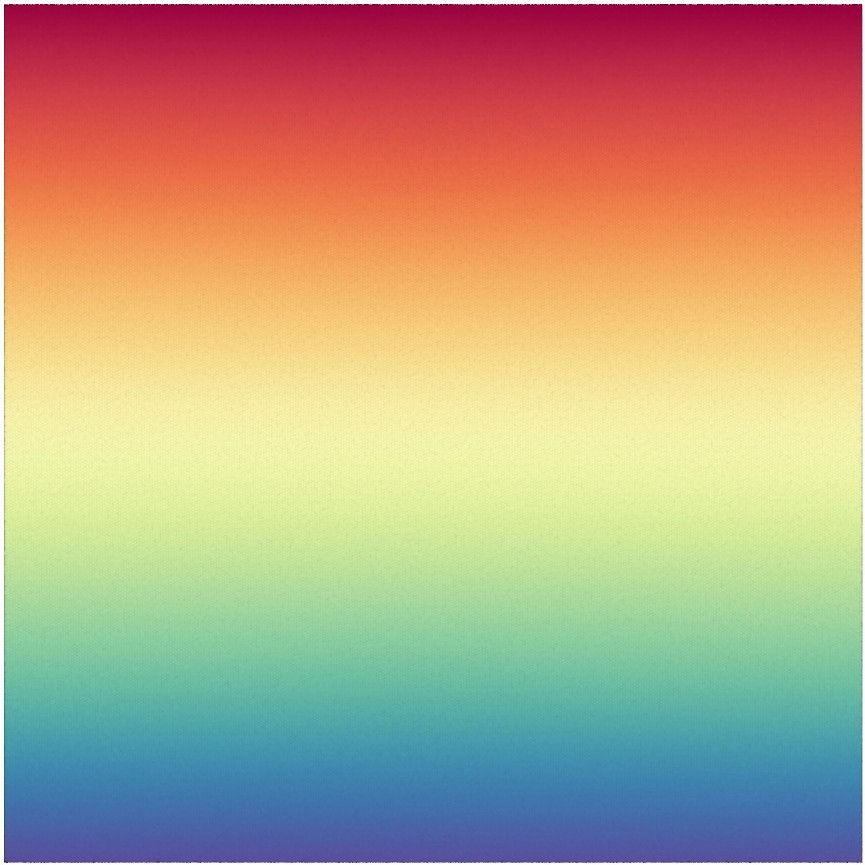
\includegraphics[width=\textwidth]{images/density/taylorgreen_t0.jpg}
    \caption{$t=0s$}
  \end{subfigure}
  \begin{subfigure}[t]{0.4\textwidth}
    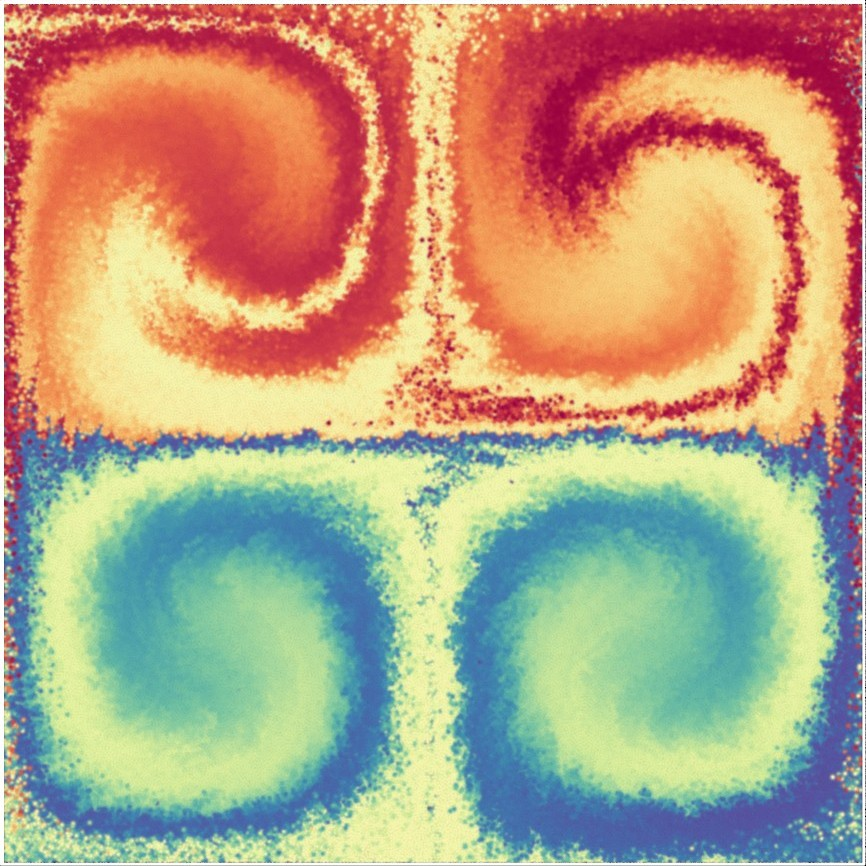
\includegraphics[width=\textwidth]{images/density/taylorgreen_t4_70.jpg}
    \caption{$t=4.7s$}
  \end{subfigure}
  \caption{$95 500$ colour coded particles are advected by a Taylor-Green vortex on a $[0;2\pi]$ domain, with four vertices each spinning in directions opposite to their respectivly adjacent vortices.}
  \label{fig:taylor-green-vortex}
\end{figure}

The rate at which the velocity of the Taylor-Green vortex on a periodic domain decays in relation to the viscosity of a fluid is analytically known to be in $\mathcal{O}br{e^{-\nu t}}$\autocite*{taylor-green-arxiv}. Despite this instance not exactly being a Taylor-Green vortex and the exact analytic solution not holding, the scenario still allows the comparison of decay of the average kinetic energy in the system for different initial samplings of the fluid, where a slower decay is more desireable in reaching lower effective viscosities. A $\frac{1}{N}E_{kin}(t)$ curve can be plotted for different initial sampling lattices and amounts of jitter in conjunction with uniform initial density, as seen in \autoref{fig:taylor-green-result}


\begin{figure}
  \centering
  \includegraphics*[width=\textwidth]{images/density/taylor-green-results.png}
  \caption*{\begin{tiny}$\nu=\nu_2=0, k=1000, \lambda=0.1, N=90500K, \vec{x}\in[0;2\pi]^2, v_{x_0} = 2\sin (x)\cos (y), v_{y,0} = -2\cos (x)\sin (y), \rho_0 = 1$ \texttt{SplitSPH}\end{tiny}}
  \caption{Time evolution of $E_{kin}$ in Taylor-Green vortex for varying amounts of initial jitter and initial sampling lattices. As the initial Jitter approaches a standard deviation of 5\% of the particle spacing, there is a continuous decrease in undesired viscosity. The hexagonal lattice being the most stable in many a sense is detrimental in this case, where to achieve low viscosities, a small jitter and a initial square-lattice sampling seem more effective.}
  \label{fig:taylor-green-result}
\end{figure}

\begin{samepage}


  \autoref{fig:taylor-green-result} suggests that viscosity does in fact decrease as the mass density varies more intensly, at least up to a reasonable amount of initial jitter.
  In order to empirically examine whether this is actually due to fewer rigid, crystalline structures forming, a metric for the degree of crystallinity or amourphousness of a material is required. For this, a metric from the study of two-dimensional melting in condensed matter physics may be borrowed: the Nelson-Halperin 2D bond orientational order parameter\autocite*{bond-orientational-parameter-pis-6} $\Psi_6$. It is defined as\autocite{nicer-psi-6-bond-orientational}:
  \begin{equation}
    \Psi_6^k = \frac{1}{6} \sum_{l\in\mathcal{N}(k)}e^{6i\Theta_{k,l}}
  \end{equation}
  where the sum is over the six nearest neighbours $k\neq l$ to the particle of index $k$, $\Theta_{k,l}$ is the angle between particles $k,l$ measured from an arbitrary, fixed axis and the index $i$ was avoided to not cause confusion with the imaginary unit in the exponent \autocite*{nicer-psi-6-bond-orientational}. Basically, crystals mostly form in hexagonal lattices in two dimensions since in this dimensionality, it is the unique closest packing - how close to crystalline a material is can therefore be measured by how close on average the angles between neighbouring particles are to forming a hexagon. The value $0 \leq \abs{\Psi_6} \leq 1$ is maximized for a hexagonal grid and decreases as the material becomes less 'well-packed'\autocite*{nicer-psi-6-bond-orientational}.

  If there was a relation between jittered masses, lower viscosity and preventing crystal structures, one would expect the average magnitude of the bond orientation parameter $\Psi_6^{avg} = \frac{1}{N}\sum_i \abs{\Psi_6^i}$ to decrease as the jitter increases and the material becomes more disorderly. To test this, $\Psi_6^{avg}$ was measured at $t=30$ for all of the configurations in \autoref{fig:taylor-green-result}, as long as possible after the initialization:

  \begin{center}
    \begin{tabular}{|c | c || c|}
      \hline
      Lattice   & Jitter $\sigma$ & $\Psi_6^{avg}$ \\ [0.5ex]
      \hline\hline
      Hexagonal & 0               & 0.522          \\\hline
      Hexagonal & 0.01h           & 0.511          \\\hline
      Hexagonal & 0.05h           & 0.459          \\\hline
      Square    & 0.01h           & 0.478          \\\hline
      Square    & 0.05h           & 0.444          \\\hline
    \end{tabular}
  \end{center}
\end{samepage}

As can be seen, irrespective of which lattice is used to sample the fluid, there are more defects, less order and therefore lower values of $\Psi_6^{avg}$ as the jitter increases, even long after the initial conditions should have no more bearing on the behaviour of the fluid.

In sources on melting of condensed matter in two dimensions, the hexatic phase is discussed, creating a middle ground between the solid and liquid phases and bearing a surface-level resemblance to structures as seen in \autoref{fig:natural-hexagons} - it might be interesting to draw from knowledge about these physical processes in order to combat undesired visocsity in SPH fluid simulation and reach higher Reynolds numbers, analysing for example the time evolution of translational and orientational order throughout a simulation and how masses and kernel support radii that vary per particle or resampling of fields can influence these phenomena - however those analyses are not conducted in this report.

Instead of focusing on $\Psi_6$ as a metric, the Vornoi tesselation of the particle configuration could also be analysed, counting for example the distribution of particles with five, six or seven nearest neighbours - generally, more amorphous structures that may better physically represent a fluid would be expected to less often have a hexagon as their associated Vornoi cell. On the other hand, especially for small kernel support radii, the SPH approximation quality might suffer from excessive particle disorder.
